\documentclass[journal]{IEEEtran}
\usepackage[utf8]{inputenc}
\usepackage[T1]{fontenc}
\usepackage{amsmath,amssymb,bm}
\usepackage{graphicx}
\usepackage{booktabs}
\usepackage{cite}
\usepackage{url}
\usepackage{balance}

\markboth{}{}

\title{ZERRE (Model H): Wave-Optics Design, Physical Synthesis, and Physics-Aware Training of a Common-Path Optoelectronic Processor}

\author{Hamza~Solak%
\thanks{H.~Solak is an independent researcher in T\"urkiye (e-mail: eng.hamzasolak@gmail.com; ORCID: 0009-0004-7541-9620).}}

\begin{document}
\maketitle

\begin{abstract}
Programmable optical neural processors often rely on expensive spatial light modulators and dual-arm interferometers that suffer from sub-wavelength vibration sensitivity. This numerical design and wave-optics simulation study presents ZERRE (Model H), an open-source common-path optoelectronic architecture built around commodity monochrome masked stereolithography (mSLA) liquid-crystal displays. Guided by measured nematic scattering attenuation, volumetric nematic reservoirs were rejected due to thermal Rayleigh--Gans scattering (15 to 40 dB/cm), and passive-matrix ITO addressing was shown via the Alt--Pleshko bound to compress usable E7 phase retardation from 4.86 rad (1.00--5.00 V) to 0.921 rad for 16 rows. An analytical Wirtinger-adjoint backpropagation operator through scalar Angular Spectrum propagation and coupled Jones modulation (relative finite-difference error $5.52 \times 10^{-7}$) enables Physics-Aware Training (PAT) against unmodeled hardware perturbations. Across three random seeds ($N_{\mathrm{test}} = 1000$) in an 8$\times$8 detector-bottlenecked regime, PAT improves linear MNIST accuracy from 67.77\% to 77.57\% (+9.80 percentage points over matched random optics) while remaining 3.70 points below direct digital area pooling (81.27\%). With a 32$\times$32 readout grid and hybrid multilayer perceptron, calibrated accuracy reaches 94.37\% on MNIST and 84.20\% on Fashion-MNIST, matching raw-pixel (93.93\%, 84.47\%) and random-optics (94.20\%, 83.97\%) MLPs; blind PAT attains 77.30\% under 15-wavelength Zernike aberrations (+0.63 points over 76.67\% head-only recalibration) and retains 94.9\% under 4-bit quantization within an estimated \$784--\$959 component budget.
\end{abstract}

\begin{IEEEkeywords}
Angular spectrum method, diffractive neural networks, liquid-crystal modulators, optoelectronic computing, physics-aware training, Wirtinger adjoint.
\end{IEEEkeywords}

% ============================================================================
\section{Introduction}
% ============================================================================

In modern CMOS and GPU accelerators, 60\% to 90\% of total inference energy is spent moving weights and activations across DRAM and interconnect hierarchies rather than performing multiply-accumulate arithmetic \cite{horowitz2014computing,sze2017efficient}. Free-space and integrated optical computing architectures address this data-movement bottleneck in the analog domain: as an optical field propagates through structured diffractive or phase-modulating elements, spatial superposition executes dense linear transformations passively during its sub-nanosecond transit across a centimeter-scale cavity ($\sim 0.33\,\text{ns}$ across a $10\,\text{cm}$ optical path) \cite{wetzstein2020inference,psaltis1985optical,lin2018alloptical}.

Static 3D-printed diffractive deep neural networks ($\text{D}^2\text{NN}$) established passive inference at terahertz wavelengths \cite{lin2018alloptical}, yet fixed dielectric plates cannot be reprogrammed after fabrication. Subsequent reconfigurable systems introduced nanophotonic Mach--Zehnder meshes \cite{shen2017deep}, large-scale diffractive processing units \cite{zhou2021largescale}, integrated photonic tensor cores \cite{feldmann2021parallel}, time-wavelength interleaving \cite{xu2021tops}, and hybrid optical-electronic convolutional front-ends \cite{chang2018hybrid}. Parallel efforts dating back to pocket liquid-crystal televisions \cite{yu1990lctv} and recent spatial-light vector-matrix multipliers \cite{spall2020reconfigurable} demonstrated that display hardware can serve as programmable optical weights.

Three engineering barriers still hinder accessible experimental adoption: laboratory liquid-crystal-on-silicon (LCOS) spatial light modulators cost \$8,000--\$40,000 per plane; dual-arm interferometers experience destructive fade under nanometer path shifts ($\lambda/4 \approx 133\,\text{nm}$ at $532\,\text{nm}$) \cite{shen2017deep}; and weights trained on idealized numerical models lose accuracy when deployed onto misaligned optical hardware, an effect worsened when designers overlook RMS voltage clamping in passive-matrix liquid-crystal cells.

This article presents a numerical design and wave-optics simulation study of \textbf{ZERRE (Model H)}, an open-source common-path optoelectronic processor architecture and digital twin; no physical benchtop prototype has been constructed or optically measured at this stage. Starting from volumetric bulk scattering bounds in nematic liquid crystals \cite{wu1987scattering}, eight candidate topologies (Models~A--H) are winnowed down to a planar $7\,\mu\text{m}$ thin-cell stack built from commodity monochrome mSLA 2K displays (\$40--\$60 each). Applying the Alt--Pleshko multiplexing theorem \cite{alt1974scanning} shows that $16\times 16$ passive-matrix scanning ($1/5$ voltage bias) restricts the RMS selection ratio to $1.290994$ and shrinks usable E7 phase retardation by $5.28\times$ ($4.86\,\text{rad}$ to $0.921\,\text{rad}$), motivating an active-matrix TFT-LCD or direct AC-PWM weight plane. Finally, deriving exact analytical Wirtinger-adjoint gradients through Angular Spectrum propagation enables Physics-Aware Training (PAT) \cite{wright2022pat,hughes2018insitu} on a perturbed physical plant simulator, audited across three random seeds on MNIST and Fashion-MNIST alongside mechanical, thermal, stray-light, bit-quantization, sub-aperture fill-factor, and Zernike aberration stress tests.

\begin{figure*}[!t]
  \centering
  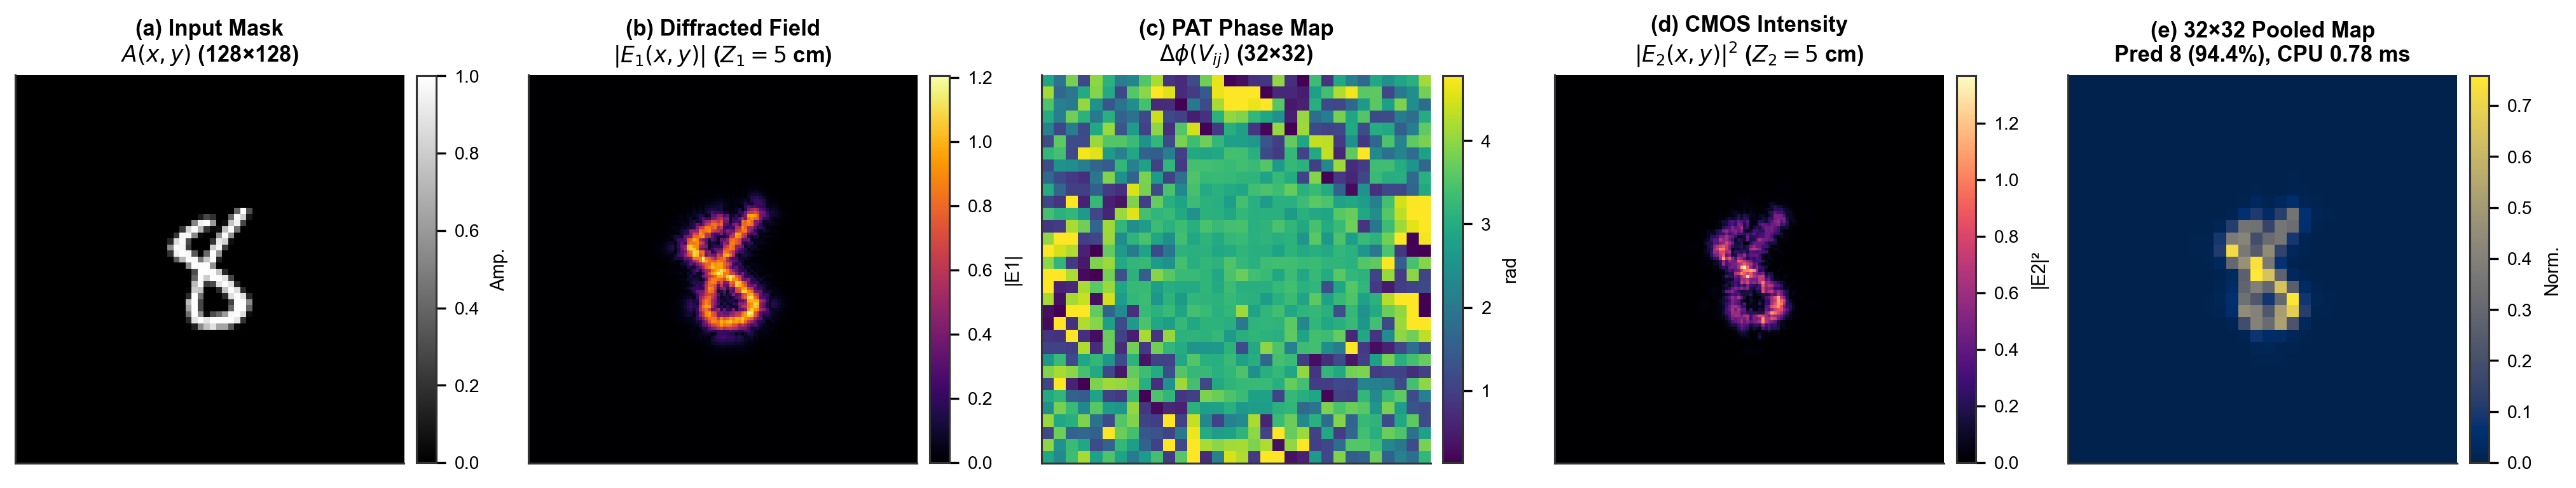
\includegraphics[width=\textwidth]{figures/makale_fig1_dalga_en.png}
  \caption{Scalar wave-optics forward propagation of a handwritten MNIST digit (``8'') through the simulated ZERRE Model H pipeline ($N=128^2$, $\Delta x=47\,\mu\text{m}$): \textbf{(a)} input amplitude mask $A(x,y)$ on the monochrome mSLA panel; \textbf{(b)} diffracted field amplitude $|E_1(x,y)|$ at the LC weight plane after $Z_1=5\,\text{cm}$ Angular Spectrum propagation; \textbf{(c)} PAT-trained $32\times 32$ active LC phase retardation map $\Delta\phi(V_{ij})$ [rad]; \textbf{(d)} CMOS sensor intensity $|E_2(x,y)|^2$ after crossed-analyzer projection and $Z_2=5\,\text{cm}$ propagation; \textbf{(e)} $32\times 32$ pooled optical feature map (predicted Class~8 at $94.4\%$ confidence; $0.78\,\text{ms}$ median CPU simulation time on $N=128^2$).}
  \label{fig:wave_chain}
\end{figure*}

% ============================================================================
\section{Architectural Synthesis and Physical Constraints}
% ============================================================================

\subsection{Bulk Nematic Scattering: Spherical Reservoir vs. Thin Planar Cell}
Among eight evaluated conceptual topologies (Models~A--H), four volumetric nematic-reservoir designs (32-electrode Fibonacci sphere Model~A, hemispherical hybrid bowl Model~C, photodiode-addressed sphere Model~F, and spherical ITO matrix Model~G) investigated filling centimeter-scale borosilicate vessels ($\varnothing 100\,\text{mm}$) with Merck E7 to induce three-dimensional optical mixing. In nematic mesophases, however, thermal fluctuations of the molecular director generate Rayleigh--Gans scattering roughly two orders of magnitude stronger than intrinsic absorption, producing attenuation coefficients of $\alpha_{\mathrm{scat}} \approx 15\text{--}40\,\text{dB/cm}$ across the visible spectrum \cite{wu1987scattering}. Across a $L = 10\,\text{cm}$ optical path inside a spherical cell, ballistic attenuation reaches $150\text{--}400\,\text{dB}$, extinguishing wavefront coherence into diffuse photon transport and rendering the director field unstable under mechanical sloshing.

By contrast, confining E7 inside a planar gap of $d \le 7\,\mu\text{m}$ reduces bulk scattering loss to $0.003\text{--}0.03\,\text{dB}$ while capillary forces immobilize the fluid layer. At $\lambda = 532\,\text{nm}$, a $7\,\mu\text{m}$ layer of pure E7 ($\Delta n = 0.225$) imparts an unbiased phase retardation of $18.60\,\text{rad}$ ($\approx 5.92\pi$), spanning multiple interference orders. A monotonic, single-order working window of
\begin{equation}
  \Delta\phi_{\max} = \frac{2\pi}{\lambda}\,\Delta n_{\mathrm{eff}}\, d \approx 4.97\,\text{rad} \; (\approx 1.58\pi)
  \label{eq:max_phase}
\end{equation}
is realized either with fluorinated nematic mixtures native to mSLA TFT panels ($\Delta n_{\mathrm{eff}} \approx 0.060$ at $d = 7\,\mu\text{m}$), a thinner $d = 1.87\,\mu\text{m}$ pure E7 gap, or a $7\,\mu\text{m}$ E7 cell biased above $2.2\,\text{V}$ RMS. Among the remaining planar thin-cell candidates, a passive $16\times 16$ ITO plate (Model~B) encounters the multiplexing limit analyzed in Section~II-C, a single 7-layer stack (Model~D) defines the $7\,\mu\text{m}$ cell cross-section, and a 3-layer cascaded stack (Model~E) compounds insertion loss and alignment tolerances, leaving the single-weight-plane common-path stack (Model~H) as the minimal realizable synthesis. Any future exploratory test of thick-cell scattering is gated by a low-cost $1\,\text{cm}$ glass cuvette transmission check prior to spherical fabrication.

\subsection{Input Encoding via Commodity mSLA Monochrome LCDs}
Mass-produced monochrome LCD panels built for masked stereolithography (mSLA) 3D printers offer a practical alternative to research LCOS modulators. Typical units offer $1440\times 2560$ pixels on a $5.5\,\text{inch}$ panel ($\sim 47\,\mu\text{m}$ pitch, with $1620\times 2560$ resolution on $\sim 6.1\,\text{inch}$ displays), omit absorptive RGB color filters, ship without a backlight as bare transmissive valves, and interface with standard HDMI-to-MIPI driver boards at $60\,\text{Hz}$ (8-bit grayscale) for \$40--\$60. Although thin-film transistor (TFT) bus lines restrict clear aperture transmittance to roughly 4\%--8\%, a $100\,\text{mW}$ $532\,\text{nm}$ diode-pumped solid-state (DPSS) laser paired with millisecond camera exposure easily compensates for this loss, while the $16.7\,\text{ms}$ frame refresh outpaces the $\sim 50\,\text{ms}$ viscoelastic relaxation time of E7.

\begin{figure*}[!t]
  \centering
  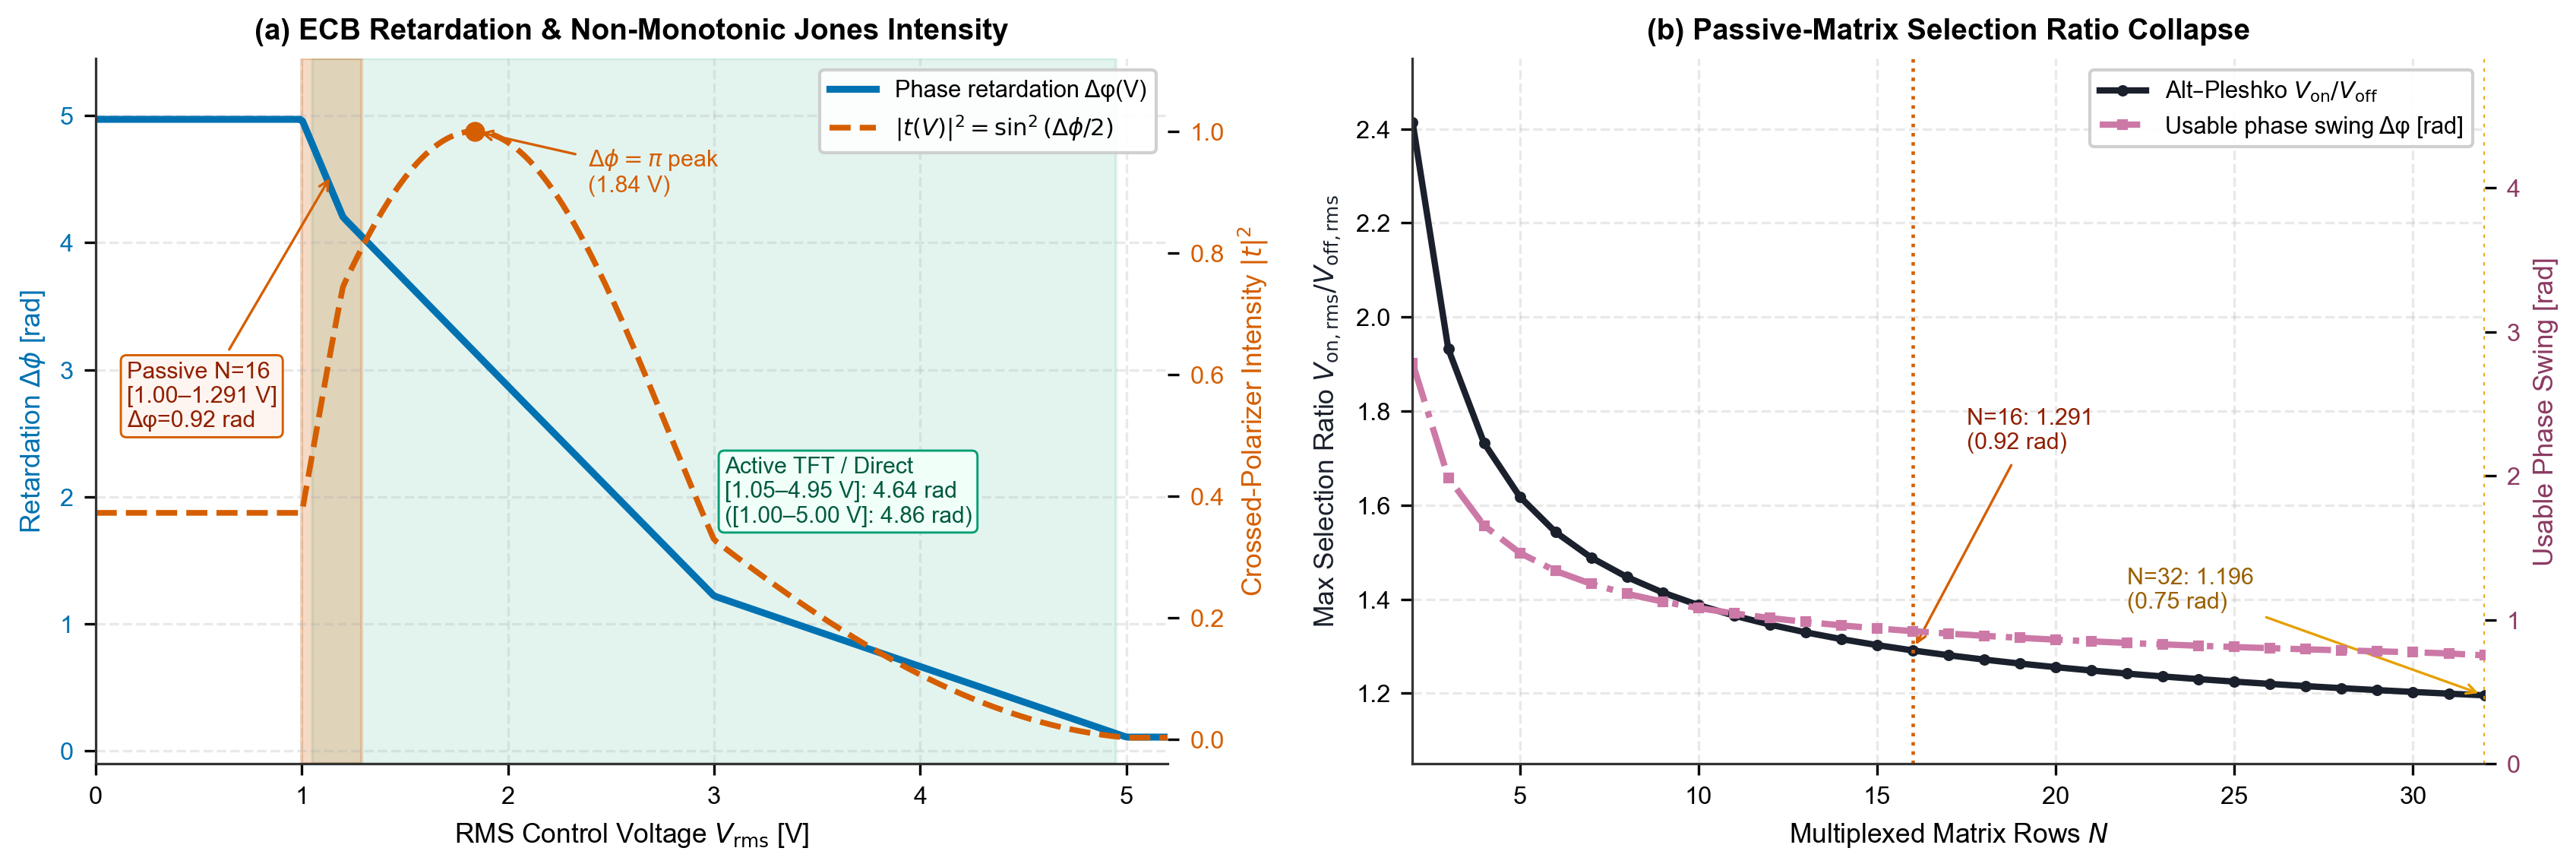
\includegraphics[width=0.96\textwidth]{figures/makale_fig2_alt_pleshko_en.png}
  \caption{Passive-matrix multiplexing limit in nematic LC weight layers: \textbf{(a)}~ECB phase retardation $\Delta\phi(V_{\mathrm{rms}})$ (blue, left axis) and non-monotonic crossed-polarizer intensity transmittance $|t(V)|^2 = \sin^2(\Delta\phi/2)$ peaking at $\Delta\phi = \pi$ near $1.84\,\text{V}$ (dashed vermilion, right axis). Red shading marks the $[1.00\,\text{V}, 1.291\,\text{V}]$ RMS window ($0.921\,\text{rad}$ swing) enforced by $16\times 16$ passive scanning versus the $4.64\,\text{rad}$ active PAT window over $[1.05, 4.95]\,\text{V}$ ($4.86\,\text{rad}$ over $[1.00, 5.00]\,\text{V}$, green). \textbf{(b)}~Alt--Pleshko maximum RMS selection ratio and usable phase swing as multiplexed row count $N$ increases from 2 to 32.}
  \label{fig:alt_pleshko}
\end{figure*}

\subsection{The Alt--Pleshko RMS Bottleneck in Passive Matrices}
Addressing an $N\times N$ ITO grid using $2N$ row-and-column channels via time multiplexing (for instance, a $1/5$ voltage bias scheme for $N=16$) appears economical at first glance. Because the electro-optic dielectric torque in a nematic LC scales quadratically with electric field ($\propto E^2$) and integrates over a $\sim 50\,\text{ms}$ response time, each cell reacts to the root-mean-square voltage over the entire scan period rather than instantaneous row pulses:
\begin{equation}
  V_{\mathrm{rms}}(i,j) = \sqrt{\frac{1}{N}\left(V_{\mathrm{sel}} + U_{ij}V_{\mathrm{data}}\right)^2 + \frac{1}{N}\sum_{r\neq i}\left(U_{rj}V_{\mathrm{data}}\right)^2},
  \label{eq:vrms}
\end{equation}
where $U_{rj}\in[-1, +1]$ denotes normalized column weights. Under optimal drive ratio $V_{\mathrm{sel}}/V_{\mathrm{data}} = \sqrt{N}$ ($=4$ for $N=16$), the Alt--Pleshko theorem \cite{alt1974scanning} bounds the maximum RMS selection ratio to
\begin{equation}
  \frac{V_{\mathrm{on,rms}}}{V_{\mathrm{off,rms}}} \le \sqrt{\frac{\sqrt{N}+1}{\sqrt{N}-1}}.
  \label{eq:alt_pleshko}
\end{equation}

For $N=16$ multiplexed rows, this ceiling equals $\sqrt{5/3} \approx 1.290994$ (dropping further to $1.195606$ at $N=32$). Holding unselected elements near the $1.00\,\text{V}$ Freedericksz threshold caps selected pixels at $1.291\,\text{V}$ RMS, reducing usable E7 phase modulation from $4.86\,\text{rad}$ down to $0.921\,\text{rad}$ ($5.28\times$ loss, Fig.~\ref{fig:alt_pleshko}a) while introducing vertical column crosstalk through the summation in \eqref{eq:vrms}. Model H therefore replaces passive row scanning in the weight plane with either direct AC-coupled PWM channels or a second commodity active-matrix TFT mSLA panel, whose pixel-level storage capacitors eliminate column crosstalk.

% ============================================================================
\section{Wave-Optics Model and Physics-Aware Training}
% ============================================================================

\subsection{Angular Spectrum Propagation and Coupled Jones Modulation}
Linearly polarized ($0^\circ$) $532\,\text{nm}$ light modulated in amplitude by the input mSLA panel forms $E_0(x,y) = A(x,y)$ and propagates across free space $Z_1 = 5\,\text{cm}$ via the non-paraxial scalar Angular Spectrum Method (ASM) \cite{goodman2017fourier}:
\begin{align}
  E_1 &= \mathcal{P}_{Z_1}\{E_0\} = \mathcal{F}^{-1}\!\left\{\mathcal{F}\{E_0\} \odot H(f_x, f_y; Z_1)\right\}, \label{eq:asm} \\
  H(f_x, f_y; z) &= \exp\!\left(i\frac{2\pi}{\lambda}z\sqrt{1 - \lambda^2 f_x^2 - \lambda^2 f_y^2}\right) \cdot \mathbb{I}_{f_x^2+f_y^2 < \lambda^{-2}}, \label{eq:transfer}
\end{align}
where evanescent spatial frequencies are truncated. At the weight plane, our analytical model treats each pixel as a parallel-aligned electrically controlled birefringence (ECB) retarder oriented at $45^\circ$ between crossed polarizers ($0^\circ/90^\circ$). Up to an overall global phase, its scalar Jones transmittance is
\begin{equation}
  t(V_{ij}) = \sin\!\left(\frac{\Delta\phi(V_{ij})}{2}\right) \exp\!\left(i\frac{\Delta\phi(V_{ij})}{2}\right),
  \label{eq:jones}
\end{equation}
producing $E_2 = \mathcal{P}_{Z_2}\{E_1 \odot M(\mathbf{V})\}$ across $Z_2 = 5\,\text{cm}$ and square-law sensor intensity $I_{\mathrm{CMOS}} = |E_2|^2$, which is block-averaged over a centered $K\times K$ detector grid into $\mathbf{f} \in \mathbb{R}^{K^2}$ (Fig.~\ref{fig:wave_chain}). Notice that $\Delta\phi(V)$ follows a piecewise-linear electro-optic curve falling monotonically from $4.97\,\text{rad}$ at $1.00\,\text{V}$ to $0.11\,\text{rad}$ at $5.00\,\text{V}$ ($4.86\,\text{rad}$ full span; $4.64\,\text{rad}$ within the PAT active bounds $[1.05, 4.95]\,\text{V}$), whereas the intensity factor $|t(V)|^2 = \sin^2(\Delta\phi/2)$ is non-monotonic and peaks at $\Delta\phi = \pi$ (Fig.~\ref{fig:alt_pleshko}a). Here \eqref{eq:jones} acts as a closed-form coupled amplitude--phase surrogate for commercial twisted-nematic (TN) mSLA displays \cite{lu1990lctv}; physical assembly using a TN weight panel requires aligning its polarizers appropriately and empirically calibrating its voltage--Jones curve. Forward and adjoint FFT propagations during PAT execute in \texttt{complex64} precision, whereas non-PAT analytical sweeps and evaluation paths run in \texttt{complex128}.

With pixel pitch $\Delta x = 47\,\mu\text{m}$, the critical ASM sampling dimension is $N_{\mathrm{crit}} = \lambda Z_1 / \Delta x^2 \approx 12.0$ pixels, so a $N=128$ (or $256$) grid satisfies Nyquist sampling by more than an order of magnitude. Maximum diffraction walk-off across $Z_1$ is $Z_1\lambda/(2\Delta x) = 0.283\,\text{mm}$, well within the zero-padded spatial guard bands of $1.69\,\text{mm}$ around the $2.63\,\text{mm}$ input digit and $0.75\,\text{mm}$ around the $4.51\,\text{mm}$ active weight array at $N=128$ ($2.73\,\text{mm}$ and $1.50\,\text{mm}$ at $N=256$), suppressing circular wrap-around aliasing.

\subsection{Analytical Wirtinger Adjoint Backpropagation}
To differentiate a scalar task loss $\mathcal{L}$ with respect to the control voltages $\mathbf{V}$ without finite-difference evaluations across hundreds of electrodes, the complex Wirtinger error field at the sensor plane for $I = E_2 E_2^*$ is written as
\begin{equation}
  G_{\mathrm{cam}} = 2 \left(\frac{\partial \mathcal{L}}{\partial I}\right) \odot E_2.
  \label{eq:wirtinger}
\end{equation}
Under the discrete real inner product $\langle u, v \rangle = \operatorname{Re}\sum u^* v$, the exact Hermitian adjoint of ASM propagation is backward propagation by $-Z_2$:
\begin{equation}
  G_{\mathrm{mask}} = \mathcal{P}_{Z_2}^{\dagger}\{G_{\mathrm{cam}}\} = \mathcal{F}^{-1}\!\left\{\mathcal{F}\{G_{\mathrm{cam}}\} \odot H^*(f_x, f_y; Z_2)\right\}.
  \label{eq:adjoint}
\end{equation}
Integrating $G_{t,ij} = \sum_{(u,v)\in\Omega_{ij}} E_1^*(u,v) G_{\mathrm{mask}}(u,v)$ over each electrode macro-pixel $\Omega_{ij}$ and applying $dt/d\phi = \frac{1}{2}e^{i\phi}$ yields the exact closed-form voltage gradient in one inverse-and-forward FFT pair:
\begin{equation}
  \frac{\partial \mathcal{L}}{\partial V_{ij}} = \operatorname{Re}\!\left\{G_{t,ij}^* \cdot \frac{1}{2}e^{i\Delta\phi(V_{ij})}\right\} \cdot \left.\frac{d\Delta\phi}{dV}\right|_{V_{ij}}.
  \label{eq:grad_v}
\end{equation}
Against central finite differences ($\varepsilon = 10^{-6}$), \eqref{eq:grad_v} agrees to a relative $L_2$ error of $5.52 \times 10^{-7}$ in active mode and $7.46 \times 10^{-7}$ under the passive Alt--Pleshko RMS chain rule (Fig.~\ref{fig:ablation_pat}b).

\begin{figure*}[!t]
  \centering
  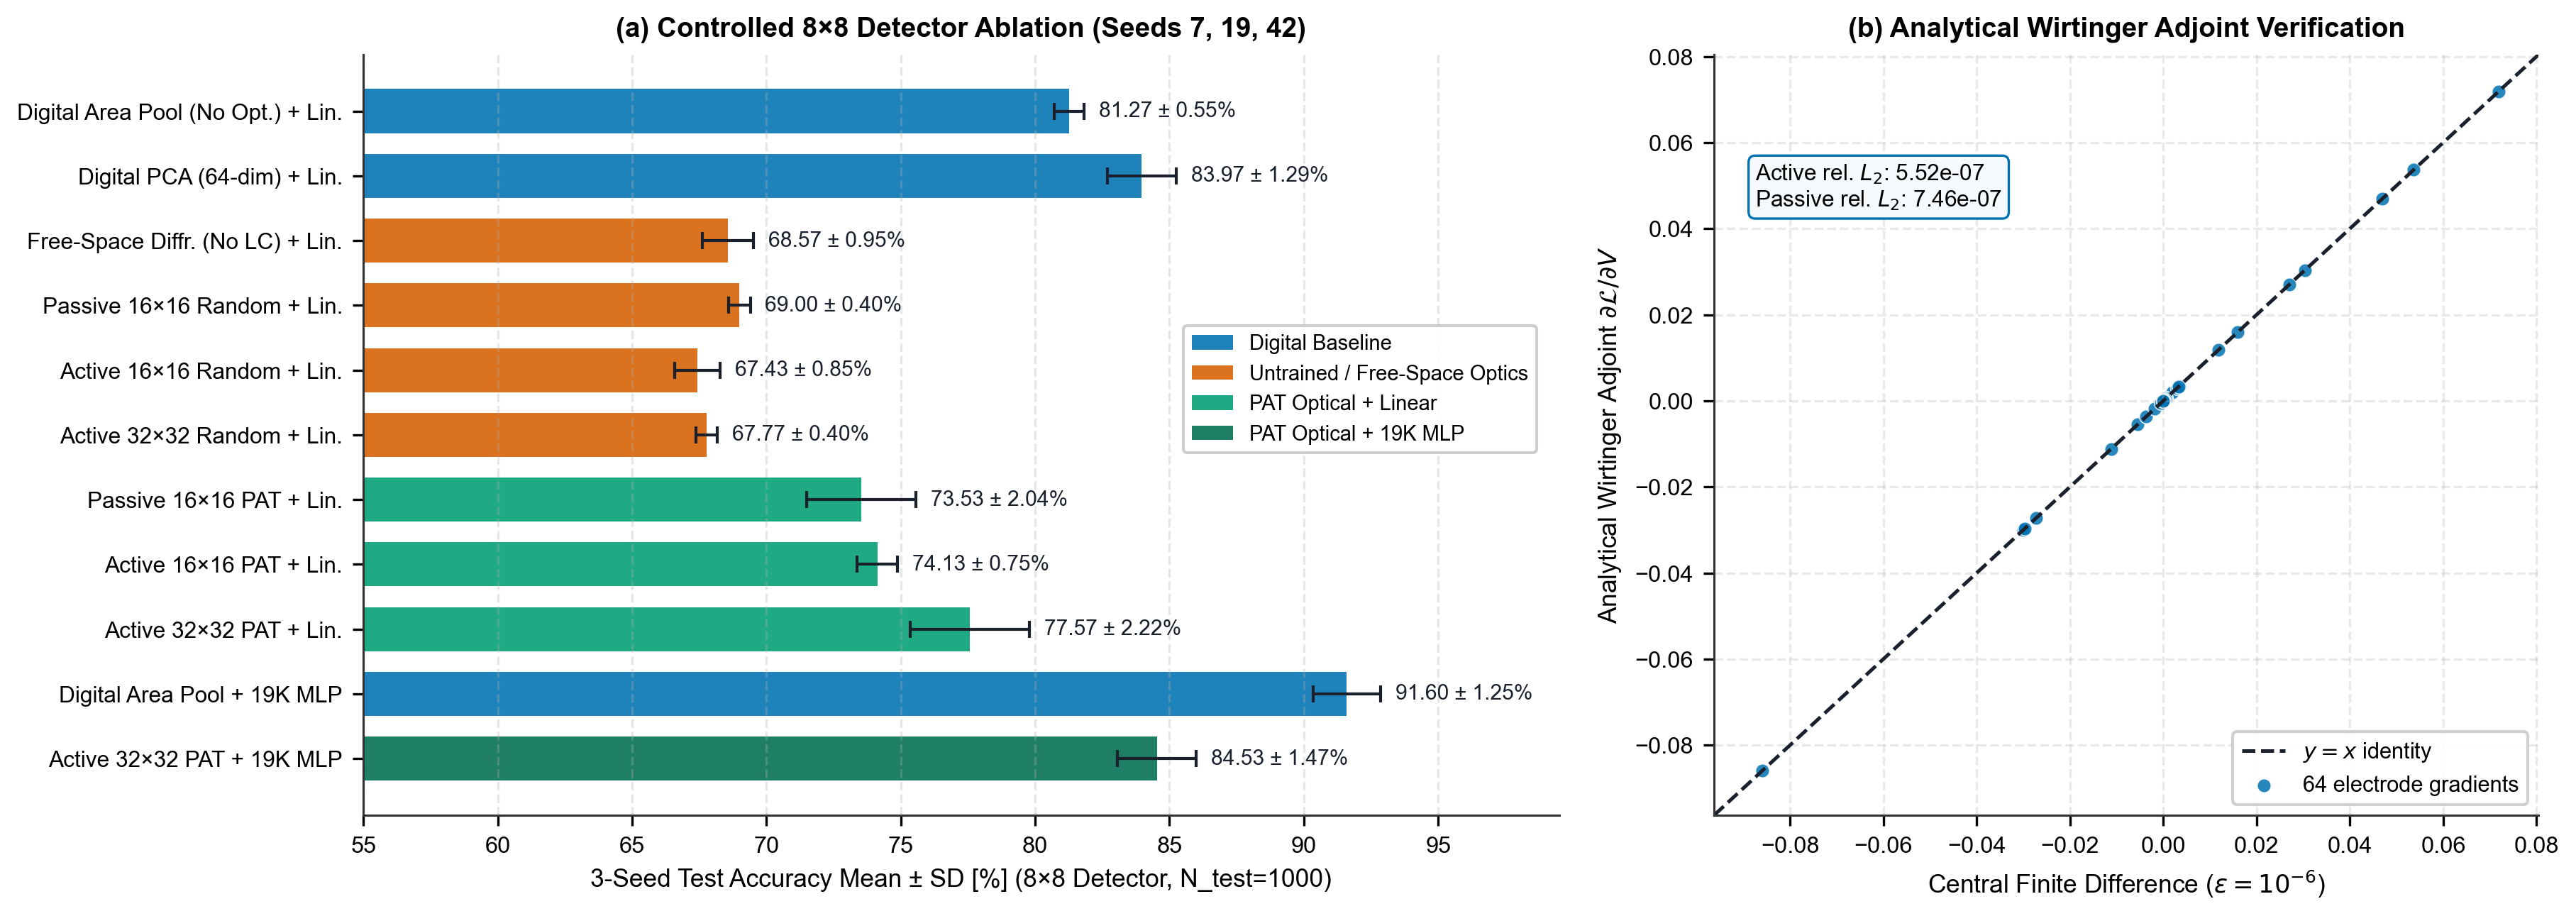
\includegraphics[width=0.98\textwidth]{figures/makale_fig3_ablasyon_pat_en.png}
  \caption{\textbf{(a)} Leakage-free 3-seed MNIST test accuracy (mean $\pm$ 1~SD, $N_{\mathrm{test}}=1000$) across all 11 matched configurations in the $8\times 8$ detector-bottlenecked regime on a perturbed physical plant simulator. PAT-trained $32\times 32$ active optics improves linear classification by $+9.80$ points over matched random optics ($77.57\%$ vs.\ $67.77\%$) while remaining $3.70$ points below direct digital area pooling ($81.27\%$). \textbf{(b)} Parameter-wise agreement between analytical Wirtinger adjoint gradients and central finite differences ($\varepsilon=10^{-6}$).}
  \label{fig:ablation_pat}
\end{figure*}

\subsection{Physics-Aware Training and Dark-Frame Stabilization}
Because physical optical builds exhibit uncalibrated mounting offsets, temperature shifts, and readout noise, our Physics-Aware Training (PAT) loop \cite{wright2022pat} evaluates forward sensor features $\mathbf{f}_{\mathrm{phys}}$ using a perturbed physical plant simulator while computing optical backward steps via \eqref{eq:wirtinger}--\eqref{eq:grad_v} on the uncalibrated nominal digital twin (retaining Simultaneous Perturbation Stochastic Approximation, SPSA \cite{spall1998spsa}, as a gradient-free fallback). Under ambient stray light, near-zero-variance peripheral CMOS pixels can blow up by orders of magnitude during z-score normalization. We suppress this instability by subtracting a 16-frame noisy dark background estimate and enforcing a training-only standard-deviation floor:
\begin{equation}
  \tilde{\mathbf{f}} = \frac{(\mathbf{f}_{\mathrm{on}} - \mathbf{f}_{\mathrm{dark}}) - \bm{\mu}_{\mathrm{tr}}}{\max\!\left(\bm{\sigma}_{\mathrm{tr}},\, 0.05\cdot\operatorname{mean}(\bm{\sigma}_{\mathrm{tr}})\right)},
  \label{eq:sd_floor}
\end{equation}
where $\bm{\mu}_{\mathrm{tr}}$ and $\bm{\sigma}_{\mathrm{tr}}$ are computed strictly from the training split without test-set leakage.

\begin{table}[!t]
  \centering
  \caption{Simulation Setup, Optical Geometry, and Training Hyperparameters}
  \label{tab:sim_setup}
  \begin{tabular}{@{}ll@{}}
    \toprule
    \textbf{Parameter} & \textbf{Value / Specification} \\
    \midrule
    Wavelength $\lambda$ / Pixel pitch $\Delta x$ & $532\,\text{nm}$ / $47\,\mu\text{m}$ \\
    Axial spacings $Z_1$, $Z_2$ & $50\,\text{mm}$, $50\,\text{mm}$ ($10\,\text{cm}$ path, $0.33\,\text{ns}$) \\
    Grid sizes $N$ & $128\times 128$ ($6.02\,\text{mm}$), $256\times 256$ ($12.03\,\text{mm}$) \\
    ASM critical grid / Walk-off & $N_{\mathrm{crit}} = 12.0\,\text{px}$ / $0.283\,\text{mm}$ \\
    Zero-pad guard bands ($N=128$) & $1.69\,\text{mm}$ (input), $0.75\,\text{mm}$ (weight) \\
    Active / Passive control bounds & $[1.05, 4.95]\,\text{V}$ ($4.64\,\text{rad}$) / $[-1, +1]$ ($0.921\,\text{rad}$) \\
    Optimizer & Adam ($\text{lr}_{\mathrm{opt}}=0.07\text{--}0.10$; $\text{lr}_{\mathrm{head}}=2.5\times 10^{-2}$ / $2.5\times 10^{-3}$) \\
    Regularization / Schedule & $10^{-4}$ $L_2$; $16\text{--}22$ ep.\ (PAT), $40\text{--}45$ ep.\ (MLP); early stop \\
    Perturbed plant faults & $47\,\mu\text{m}$ LCD/CMOS, $+1.2$/$-0.8\,\text{mm}$ $Z$, $29\,^\circ\text{C}$, $2\%$ drift \\
    Evaluation seeds / Test count & $\{7, 19, 42\}$ / $N_{\mathrm{test}}=1000$ per split \\
    \bottomrule
  \end{tabular}
\end{table}

% ============================================================================
\section{Numerical Results and Analysis}
% ============================================================================

\subsection{Controlled 8$\times$8 Detector Ablation on MNIST}
All numerical experiments were executed in Python~3.11.9 / NumPy~2.2.3 on CPU (Intel64 Family 6 Model 170) using \texttt{complex64} propagation in PAT paths and \texttt{complex128} in non-PAT/evaluation paths under Table~\ref{tab:sim_setup}. To isolate what programmable optical weights contribute when electronic readout bandwidth is severely constrained, we benchmarked 11 matched configurations over an $8\times 8 = 64$ detector grid on MNIST \cite{lecun1998mnist} across three random seeds ($N_{\mathrm{fit}} = 2640$, $N_{\mathrm{val}} = 360$, $N_{\mathrm{test}} = 1000$). The plant simulator included $47\,\mu\text{m}$ lateral LCD and sensor shifts, $+1.2\,\text{mm}/-0.8\,\text{mm}$ axial spacing errors, a $29\,^\circ\text{C}$ Haller thermal birefringence drift \cite{haller1975thermodynamic,li2005lc}, 2\% laser gain drift, and Gaussian readout noise, all unknown to the surrogate twin (Table~\ref{tab:ablation}, Fig.~\ref{fig:ablation_pat}a).

\begin{table}[!t]
  \centering
  \caption{Controlled MNIST Ablation on Perturbed Plant ($8\times 8$ Detector, 3 Seeds, $N_{\mathrm{test}}=1000$)}
  \label{tab:ablation}
  \begin{tabular}{@{}llrrr@{}}
    \toprule
    \textbf{\#} & \textbf{Architecture / Configuration} & \textbf{Opt. W} & \textbf{Dig. W} & \textbf{Test (\%)} \\
    \midrule
    1 & Digital Area Pooling ($8\times 8$) + Linear & 0 & 650 & $81.27 \pm 0.55$ \\
    2 & Digital PCA Basis ($64$-dim) + Linear & 0 & 650\rlap{\textsuperscript{a}} & $83.97 \pm 1.29$ \\
    3 & Free-Space Diffraction Only (No LC) & 0 & 650 & $68.57 \pm 0.95$ \\
    4 & Passive $16\times 16$ Random + Linear & 256 & 650 & $69.00 \pm 0.40$ \\
    5 & Active $16\times 16$ Random + Linear & 256 & 650 & $67.43 \pm 0.85$ \\
    6 & Active $32\times 32$ Random + Linear & 1,024 & 650 & $67.77 \pm 0.40$ \\
    7 & Passive $16\times 16$ + PAT + Linear & 256 & 650 & $73.53 \pm 2.04$ \\
    8 & Active $16\times 16$ + PAT + Linear & 256 & 650 & $74.13 \pm 0.75$ \\
    \textbf{9} & \textbf{Active $32\times 32$ + PAT + Linear} & \textbf{1,024} & \textbf{650} & \textbf{77.57 $\pm$ 2.22} \\
    10 & Digital Area Pooling ($8\times 8$) + MLP & 0 & 19,210 & $91.60 \pm 1.25$ \\
    \textbf{11} & \textbf{Active $32\times 32$ + PAT + MLP} & \textbf{1,024} & \textbf{19,210} & \textbf{84.53 $\pm$ 1.47} \\
    \bottomrule
  \end{tabular}
  \\[2pt]\footnotesize{\textsuperscript{a}Excludes the $784\times 64$ linear PCA projection matrix fit on training data.}
\end{table}

Two clear trends emerge from Table~\ref{tab:ablation}. First, unoptimized diffraction degrades accuracy sharply relative to direct imaging onto an $8\times 8$ pixel sensor ($67.77\%$--$69.00\%$ vs.\ $81.27\%$) because free-space divergence spreads localized strokes across coarse pixels. Optimizing the $32\times 32$ active LC weights with PAT recovers $+9.80$ percentage points over matched $32\times 32$ random optics ($67.77\% \to 77.57\%$) and $+9.00$ points over bare free-space propagation ($68.57\%$). By contrast, at $16\times 16$ optical resolution, passive PAT ($73.53 \pm 2.04\%$) and active PAT ($74.13 \pm 0.75\%$) are statistically equivalent within one standard deviation because the $8\times 8$ readout remains bottlenecked by detector rank rather than phase stroke. Second, a single programmable diffractive layer operating on positive square-law intensity still lags behind direct electronic $8\times 8$ area pooling ($77.57\%$ vs.\ $81.27\%$, and $84.53\%$ vs.\ $91.60\%$ with a 19K-parameter MLP), while a data-driven linear PCA-64 projection sets the unconstrained linear ceiling at $83.97 \pm 1.29\%$. Single-plane optics learns a task-aligned spatial kernel relative to random wave mixing, but does not outcompute noiseless digital spatial pooling by itself.

\subsection{Full-Scale 32$\times$32 Hybrid Classification on MNIST and Fashion-MNIST}
Scaling the CMOS detector grid to $32\times 32$ ($1,024$ pooled features) reveals how optical and electronic capacities interact across both MNIST \cite{lecun1998mnist} and 10-class Fashion-MNIST \cite{xiao2017fashion} (Table~\ref{tab:scaling}). With a regularized Ridge linear readout at $N_{\mathrm{train}}=6000$, a fixed random $32\times 32$ optical mask outperforms raw $28\times 28$ digital pixels on MNIST ($85.57 \pm 1.76\%$ vs.\ $82.93 \pm 1.70\%$), whereas PAT-trained $32\times 32$ Ridge on Fashion-MNIST is comparable to raw digital pixels within one standard deviation ($79.50 \pm 0.80\%$ vs.\ $79.07 \pm 0.81\%$).

\begin{table}[!t]
  \centering
  \caption{Full-Scale $32\times 32$ Hybrid \& Digital Baselines (3 Seeds, $N_{\mathrm{test}}=1000$)}
  \label{tab:scaling}
  \begin{tabular}{@{}lrrrr@{}}
    \toprule
    \textbf{Configuration} & \textbf{Opt. W} & \textbf{Dig. W} & \textbf{MNIST (\%)} & \textbf{F-MNIST (\%)} \\
    \midrule
    Raw $28\times 28$ Digital Ridge ($N=6\text{k}$) & 0 & 7,850 & $82.93 \pm 1.70$ & $79.07 \pm 0.81$ \\
    Opt. $16\times 16$, 256f Ridge ($N=2.5\text{k}$) & 256 & 2,570 & $81.73 \pm 0.72$ & --- \\
    Opt. $16\times 16$, 1024f Ridge ($N=2.5\text{k}$) & 256 & 10,250 & $84.77 \pm 1.00$ & --- \\
    Opt. $32\times 32$ Rand., 1024f Ridge ($N=6\text{k}$) & 1,024 & 10,250 & $85.57 \pm 1.76$ & --- \\
    Opt. $32\times 32$ PAT, 1024f Ridge ($N=6\text{k}$) & 1,024 & 10,250 & --- & $79.50 \pm 0.80$ \\
    \midrule
    Raw $28\times 28$ Digital MLP ($N=6\text{k}$) & 0 & 203,530 & $93.93 \pm 0.99$ & $84.47 \pm 0.55$ \\
    $32\times 32$ Random Optics + MLP & 1,024 & 264,970 & $94.20 \pm 0.95$ & $83.97 \pm 0.86$ \\
    $32\times 32$ PAT + MLP (Perturbed) & 1,024 & 264,970 & $89.77 \pm 3.27$ & $80.80 \pm 1.15$ \\
    \textbf{$32\times 32$ PAT + MLP (Nominal)} & \textbf{1,024} & \textbf{264,970} & \textbf{94.37 $\pm$ 0.84} & \textbf{84.20 $\pm$ 0.44} \\
    \bottomrule
  \end{tabular}
\end{table}

Once a $1024\to 256\to 10$ ReLU MLP ($264,970$ digital weights) is attached, electronic capacity dominates classification accuracy: calibrated nominal PAT ($94.37\%$ MNIST, $84.20\%$ Fashion-MNIST), random fixed optics with an MLP ($94.20\%$, $83.97\%$), and raw digital pixels with an MLP ($93.93\%$, $84.47\%$) all converge within $\sim 0.5$ percentage points. Under the uncompensated perturbed plant simulator, PAT MLP scores $89.77 \pm 3.27\%$ on MNIST and $80.80 \pm 1.15\%$ on Fashion-MNIST. Conversely, in the detector-constrained $8\times 8$ Fashion-MNIST regime (Fig.~\ref{fig:realism}c), PAT linear classification again yields $+9.80$ points over random optics ($71.63 \pm 1.59\%$ vs.\ $61.83 \pm 0.72\%$), reaching $77.53 \pm 1.19\%$ with a 19K MLP versus $74.00 \pm 1.97\%$ (linear) and $81.47 \pm 1.80\%$ (MLP) for direct $8\times 8$ digital pooling.

\begin{figure*}[!t]
  \centering
  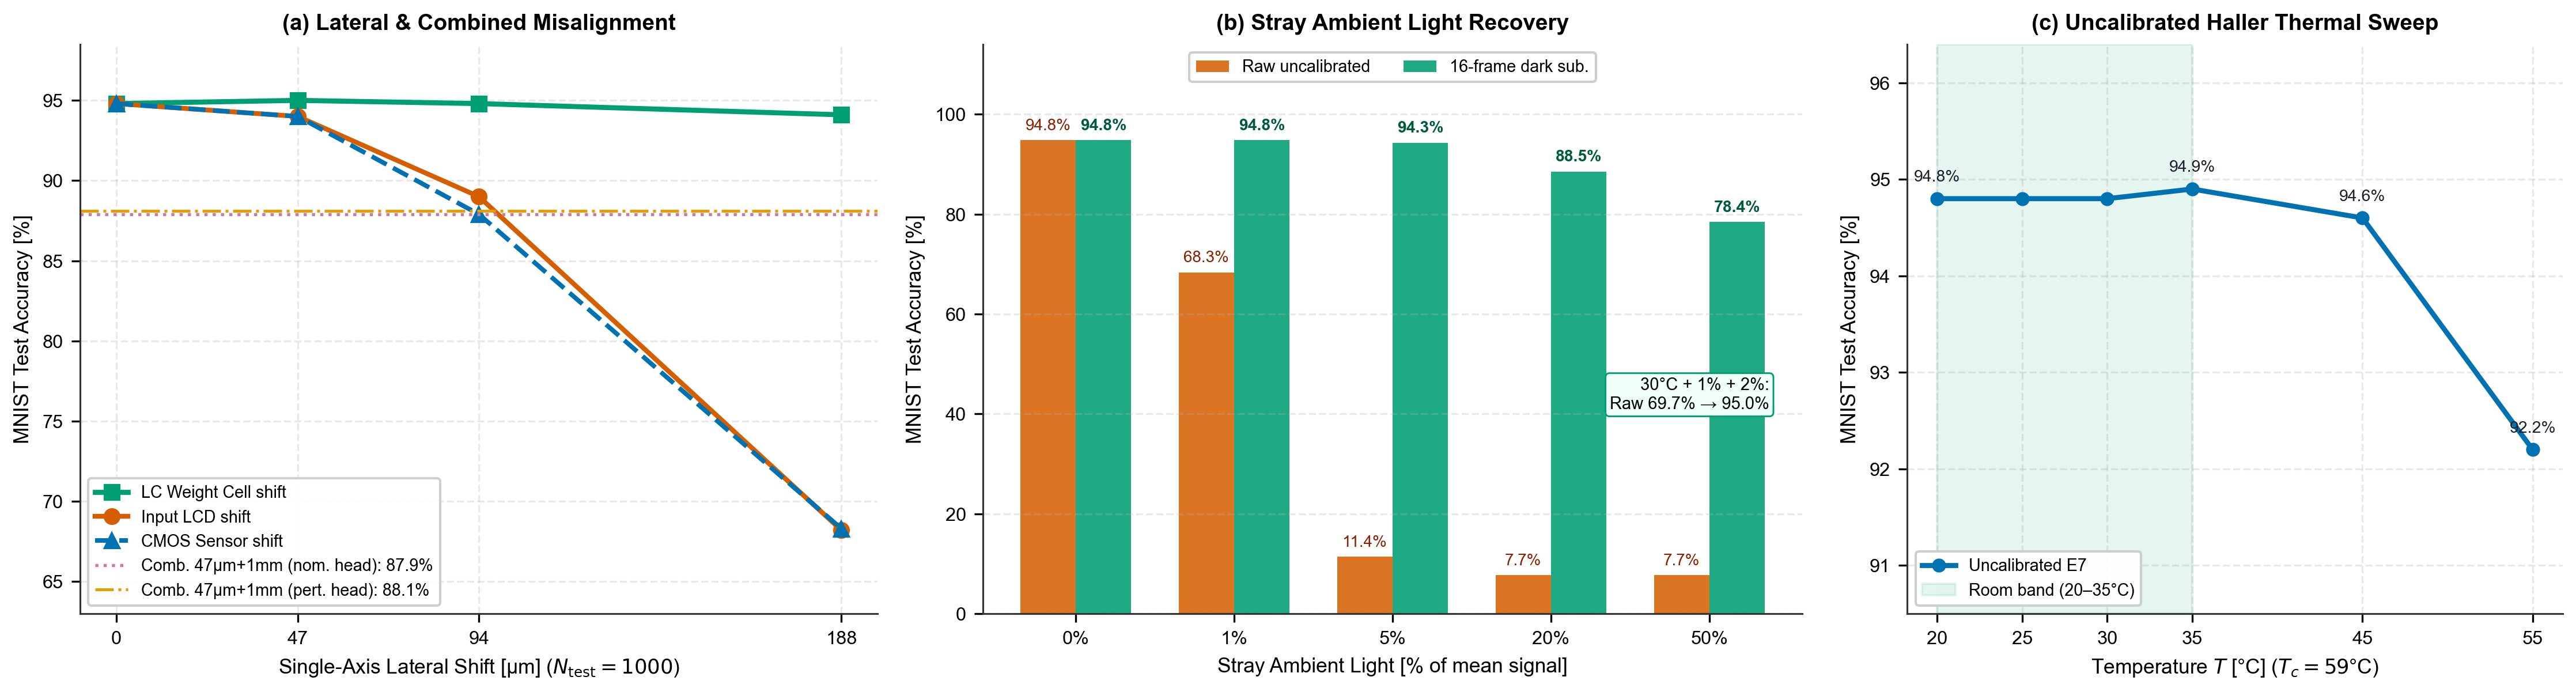
\includegraphics[width=0.96\textwidth]{figures/makale_fig4_dayanim_en.png}
  \caption{Mechanical and environmental stress tests ($N_{\mathrm{test}}=1000$, seed~7, nominal base $94.8\%$): \textbf{(a)}~single-axis lateral shifts of the LC weight cell ($94.8\% \to 94.1\%$ at $188\,\mu\text{m}$), input LCD ($94.8\% \to 68.2\%$), and CMOS sensor ($94.8\% \to 68.3\%$), alongside combined $47\,\mu\text{m} + 1\,\text{mm}$ misalignment ($87.9\%$ nominal head; $88.1\%$ perturbed-trained head from $87.8\%$ base); \textbf{(b)}~stray ambient light collapse versus 16-frame noisy dark-frame subtraction with training-only standard-deviation floor, plus $30\,^\circ\text{C} + 1\% + 2\%$ recovery ($69.7\% \to 95.0\%$); \textbf{(c)}~uncalibrated Haller thermal sweep ($20\text{--}55\,^\circ\text{C}$, $T_c=59\,^\circ\text{C}$).}
  \label{fig:robustness}
\end{figure*}

\subsection{Mechanical Alignment, Thermal Drift, and Ambient Light Resilience}
In a common-path cavity without an external reference arm, axial intensity tolerance scales with the Talbot distance $z_T = 2\Delta x^2/\lambda \approx 8.3\,\text{mm}$. Evaluated on $1,000$ MNIST test digits (seed~7, nominal base $94.8\%$, Fig.~\ref{fig:robustness}a), shifting the LC weight panel laterally up to $188\,\mu\text{m}$ incurs at most $0.7$ points loss ($94.8\% \to 94.1\%$) because incident optical fields are spatially smooth. Input LCD and CMOS sensor shifts exhibit steeper sensitivity beyond $47\,\mu\text{m}$ ($94.0\%$ at $47\,\mu\text{m}$, $68.2\%$ and $68.3\%$ at $188\,\mu\text{m}$), whereas axial shifts $\Delta Z_1 \in [0, 8\,\text{mm}]$ remain within $94.7\%$--$95.1\%$. Applying $47\,\mu\text{m}$ lateral shifts on all planes plus $+1\,\text{mm}$ axial offset lowers nominal-head accuracy to $87.9\%$ ($-6.9$ points), while a head trained directly under plant perturbations holds $88.1\%$ relative to its $87.8\%$ baseline.

Modeling E7 birefringence via the Haller power law \cite{haller1975thermodynamic,li2005lc}:
\begin{equation}
  \frac{\Delta n(T)}{\Delta n(25\,^\circ\text{C})} = \left(\frac{T_c - T}{T_c - 25}\right)^{\!\beta}, \quad T_c = 59\,^\circ\text{C},\; \beta = 0.22,
  \label{eq:haller}
\end{equation}
uncalibrated classification stays between $94.8\%$ and $94.9\%$ across $20\text{--}35\,^\circ\text{C}$, dipping to $92.2\%$ at $55\,^\circ\text{C}$ near the clearing point (Fig.~\ref{fig:robustness}c). Without background subtraction, stray ambient light totaling 1\% or 5\% of mean signal drops accuracy to $68.3\%$ and $11.4\%$. Subtracting a 16-frame noisy dark-frame estimate alongside \eqref{eq:sd_floor} maintains $94.8\%$ at 1\%, $94.3\%$ at 5\%, $88.5\%$ at 20\%, and $78.4\%$ at 50\% ambient leakage, and restores a combined $30\,^\circ\text{C}$ + 1\% leakage + 2\% laser drift fault from $69.7\%$ to $95.0\%$. Laser power variations across $\pm 10\%$ stay within $94.7\%$--$95.0\%$.

\begin{figure*}[!t]
  \centering
  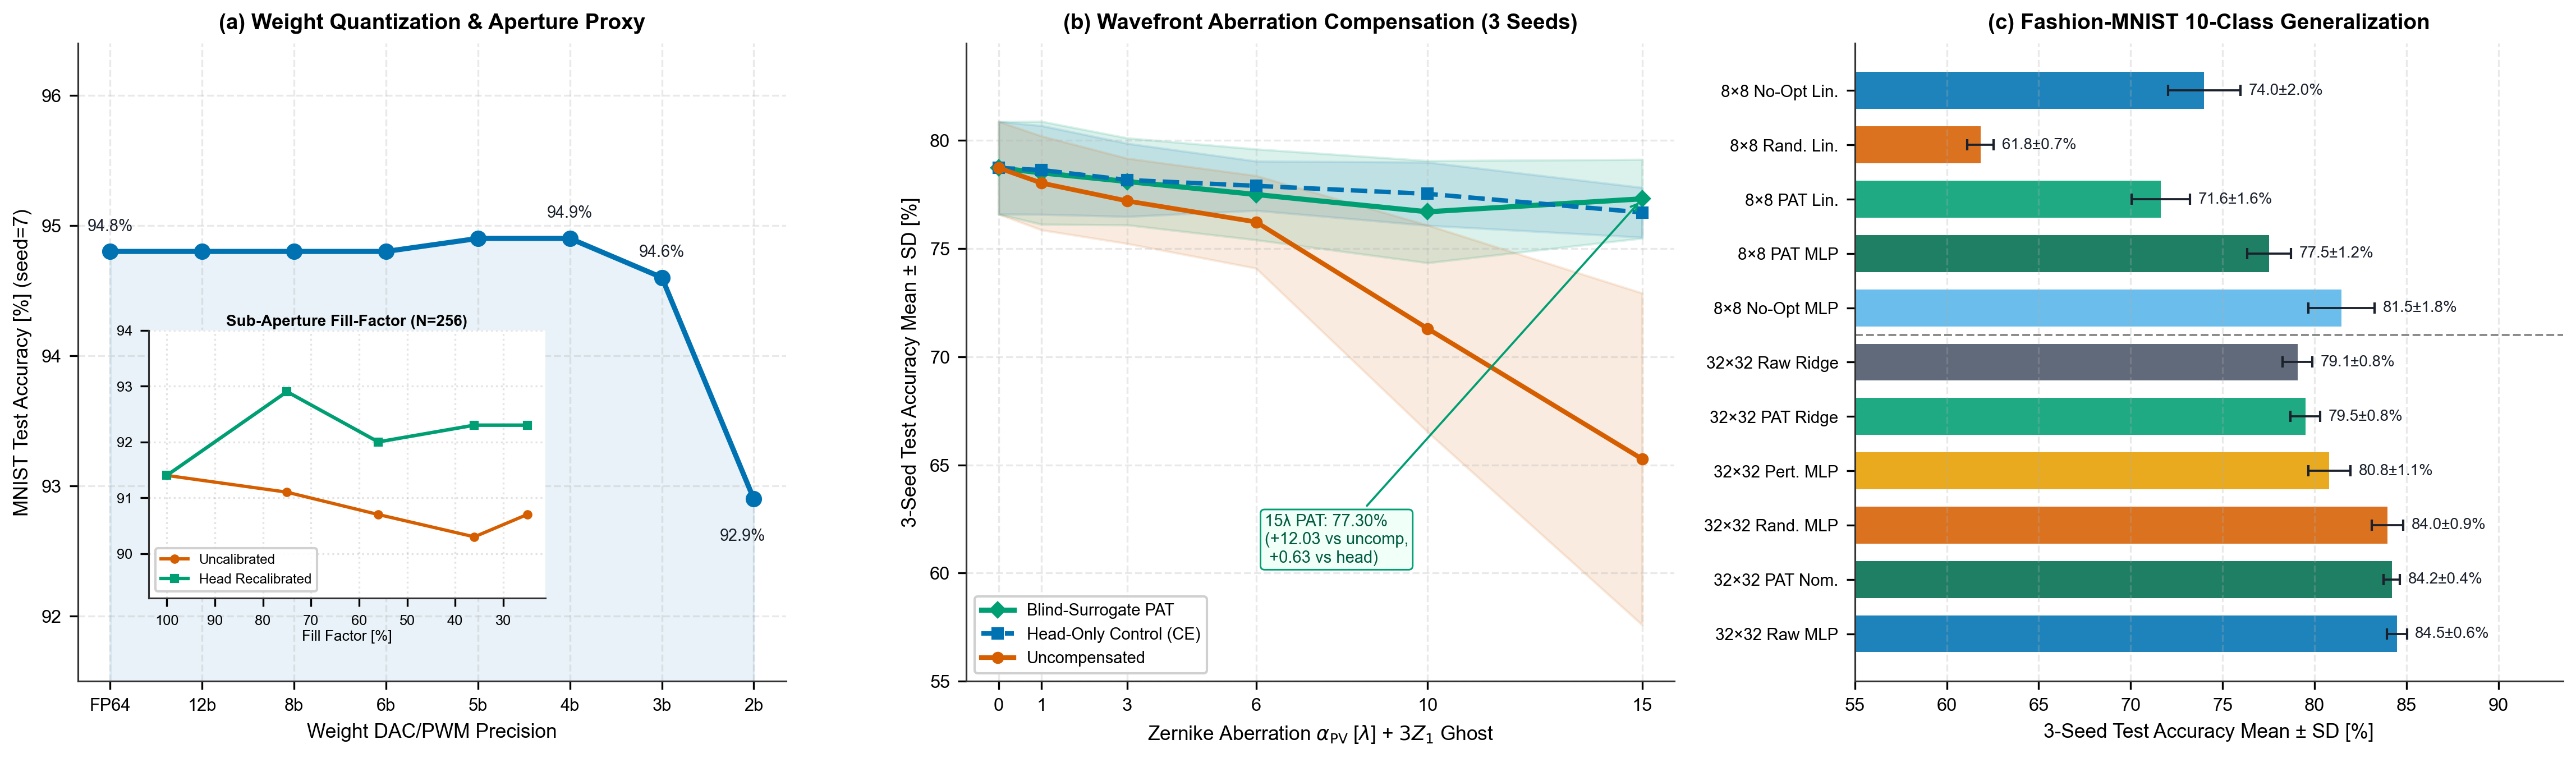
\includegraphics[width=0.98\textwidth]{figures/makale_fig5_gercekcilik_en.png}
  \caption{Hardware-realism and generalization benchmarks ($N_{\mathrm{test}}=1000$): \textbf{(a)}~post-training weight quantization with an 8-bit HDMI input panel (flat at $94.8\%$--$94.9\%$ down to 4~bits, $92.9\%$ at 2~bits) and macro-pixel sub-aperture fill-factor inset (uncalibrated $91.4\% \to 90.7\%$ vs.\ head-recalibrated $91.4\% \to 92.3\%$ at 25\% fill); \textbf{(b)}~3-seed Zernike wavefront aberrations ($0\text{--}15\lambda$ PV + $3Z_1$ ghost) comparing uncompensated weights ($65.27 \pm 7.67\%$ at $15\lambda$), matched CE head-only recalibration ($76.67 \pm 1.15\%$), and blind-surrogate PAT ($77.30 \pm 1.82\%$); \textbf{(c)}~3-seed 10-class Fashion-MNIST comparison across $8\times 8$ and $32\times 32$ regimes.}
  \label{fig:realism}
\end{figure*}

\subsection{Bit Quantization, Aperture Proxy, and Wavefront Aberrations}
Three further simulation checks test assumptions prior to benchtop fabrication (Fig.~\ref{fig:realism}a--b). Under post-training quantization of an 8-bit HDMI input coupled with $b$-bit LC control voltages (seed~7), accuracy remains constant at $94.8\%$--$94.9\%$ down to 4~bits ($16$ voltage levels), slipping modestly to $94.6\%$ at 3~bits and $92.9\%$ at 2~bits. Simulating a macro-pixel sub-aperture fill-factor proxy from $100\%$ down to $25\%$ ($N=256$ fine grid, leakage-free gain scaling) reduces uncalibrated accuracy slightly from $91.4\%$ to $90.7\%$, while recalibrating only the digital readout head stabilizes performance at $92.3\%$.

Introducing fifth-order Zernike substrate wavefront aberrations ($0\text{--}15\lambda$ peak-to-valley across defocus, astigmatism, coma, spherical aberration, and float-glass ripple) plus a $3Z_1$ Fabry--P\'erot ghost ($0.04$ Fresnel field amplitude) reveals a nuanced comparison when all conditions share identical cross-entropy Adam readout optimization (Fig.~\ref{fig:realism}b). Across $1\lambda$ to $10\lambda$, recalibrating the linear head with frozen optical weights recovers nearly all uncompensated loss ($78.03\% \to 78.63\%$ at $1\lambda$; $71.30\% \to 77.53\%$ at $10\lambda$), performing comparably to blind-surrogate PAT ($78.50\%$ and $76.70\%$). At severe $15\lambda$ distortion, uncompensated deployment falls to $65.27 \pm 7.67\%$, head recalibration alone reaches $76.67 \pm 1.15\%$, and joint optical adaptation via PAT attains $77.30 \pm 1.82\%$.

\begin{table}[!t]
  \centering
  \caption{Estimated Prototype Bill of Materials (BOM)}
  \label{tab:bom}
  \begin{tabular}{@{}llr@{}}
    \toprule
    \textbf{Subsystem} & \textbf{Selected Hardware} & \textbf{Cost (USD)} \\
    \midrule
    Optical Input & $532\,\text{nm}$ DPSS ($100\,\text{mW}$) + Expander + mSLA LCD & 150 \\
    Active Weights & 2nd mSLA TFT-LCD (or ITO Cell + AC-PWM) & 90--230 \\
    Readout \& Host & RPi Camera 3 (IMX708, $12\,\text{MP}$) + M12 + RPi 5 & 125 \\
    Optomechanics & Optical Rail, Mounts, Dark Box, $532\,\text{nm}$ Filter & 262 \\
    \midrule
    Subtotal & Core optical and electronic components & 627--767 \\
    \textbf{Total (+25\%)} & \textbf{Complete benchtop prototype w/ contingency} & \textbf{784--959} \\
    \bottomrule
  \end{tabular}
\end{table}

% ============================================================================
\section{Discussion, Limitations, and Hardware Roadmap}
% ============================================================================

Component pricing for a modular optical rail build is itemized in Table~\ref{tab:bom}, totaling \$627--\$767 in direct hardware or \$784--\$959 including a 25\% contingency margin. Three practical timescales govern such a system and must be clearly separated: passive coherent wave propagation across $10\,\text{cm}$ of optics takes $\sim 0.33\,\text{ns}$; benchtop image-by-image throughput would be paced electronically by the $60\,\text{Hz}$ LCD/camera frame interval ($\sim 16.7\,\text{ms}$) during inference and by the $\sim 50\,\text{ms}$ nematic relaxation time during weight updates; and our uncompiled NumPy CPU ASM simulator runs at a warmed median time of $0.78\,\text{ms}$ per digit ($N=128^2$, Intel64 Family 6 Model 170 CPU, Python~3.11.9 / NumPy~2.2.3, mean $0.87\,\text{ms}$, IQR $0.08\,\text{ms}$, range $0.71\text{--}2.74\,\text{ms}$ across 50 runs).

Benchtop construction introduces several engineering requirements omitted from simplified 2D models. First, a Raspberry Pi Camera Module~3 (IMX708 sensor area $6.45 \times 3.63\,\text{mm}$) is slightly smaller along its minor axis than the $4.51\text{--}6.02\,\text{mm}$ diffracted field, necessitating a $\sim 1.6\times$ demagnifying M12 relay lens pair. Second, a $100\,\text{mW}$ $532\,\text{nm}$ DPSS laser is a Class~3B source requiring OD~4+ protective eyewear, a light-tight matte enclosure, and an infrared-cut filter to reject unabsorbed $808\,\text{nm}$ and $1064\,\text{nm}$ pump leakage. Third, commodity PCA9685 PWM driver boards emit unipolar pulses that induce electrochemical degradation across bare ITO electrodes unless buffered by an AC polarity-inversion circuit, reinforcing our selection of an active TFT display backplane.

\subsection{Limitations}
Six principal limitations qualify these numerical findings and define the remaining engineering work before physical claims can be made. First, all classification accuracies and fault tolerances originate from wave-optics simulations; benchtop fabrication, optical alignment, and empirical detector noise measurements remain future work. Second, on $8\times 8$ detectors, PAT-trained optics beats matched random optics substantially ($+9.80$ points), yet still underperforms direct digital area pooling ($77.57\%$ vs.\ $81.27\%$); when a $265\text{K}$-parameter MLP head is attached at $32\times 32$, electronic capacity masks optical differences within $\sim 0.5$ points.

Third, Equation~\eqref{eq:jones} models a parallel ECB retarder as an analytical proxy, whereas twisted-nematic mSLA panels exhibit coupled polarization rotation \cite{lu1990lctv} that demands empirical lookup characterization. Fourth, our scalar simulations assume monochromatic, spatially uniform illumination, omitting DPSS laser speckle, finite coherence length, and multi-plane inter-reflections beyond the simulated $0.04$ Fabry--P\'erot ghost. Fifth, each $32\times 32$ weight block groups dozens of native $47\,\mu\text{m}$ mSLA sub-pixels, so our $N=256$ sub-aperture fill-factor test serves only as a scaled proxy rather than resolving the physical panel over a multi-thousand-pixel grid. Finally, weights tuned for one perturbed cell do not transfer directly to another cell with distinct alignment and cell-gap variations unless paired with calibration-robust objectives such as Sharpness-Aware Training \cite{sat2026pnn}.

% ============================================================================
\section{Conclusion}
% ============================================================================

Starting from bulk nematic Rayleigh--Gans attenuation ($15\text{--}40\,\text{dB/cm}$) and Alt--Pleshko RMS voltage limits ($5.28\times$ swing loss on 16-row passive grids), this study synthesized the planar common-path ZERRE (Model H) architecture around commodity mSLA panels within a \$784--\$959 prototype estimate. An exact Wirtinger-adjoint operator through scalar ASM diffraction enabled Physics-Aware Training under unmodeled mechanical, thermal, ambient-light, and aberration faults, raising $8\times 8$ linear MNIST accuracy by $+9.80$ points over random optics ($77.57\%$) and achieving $94.37\%$ MNIST and $84.20\%$ Fashion-MNIST accuracy at $32\times 32$ hybrid readout resolution, while clarifying the boundary where optical weighting adds value and identifying concrete benchtop calibration steps ahead.

% ============================================================================
\section*{Data and Code Availability}
% ============================================================================
All Python wave-optics simulation scripts (\texttt{zerre\_twin.py}, \texttt{zerre\_pat\_torch.py}), the interactive WebGL/ASM visualizer (\texttt{start\_server.py}), automated physics unit tests (\texttt{tests/test\_zerre\_physics.py}), 3-seed benchmark outputs (\texttt{makale/scripts/paper\_results.json}), and figure/manuscript generation scripts are openly released under the \textbf{MIT License} (code) and \textbf{CC BY 4.0 License} (manuscript text and figures), alongside local caching support for standard MNIST and Fashion-MNIST datasets, at \url{https://github.com/hamzasolak/zerre} (release tag \texttt{v0.4.0}; Author ORCID: \url{https://orcid.org/0009-0004-7541-9620}).

\section*{Funding}
This work was conducted as independent research without external institutional or commercial grant funding.

\section*{Conflicts of Interest}
The author declares no conflicts of interest.

\section*{Acknowledgments}
Generative AI assistance (Gemini and Claude) was used for prose editing, LaTeX formatting, and code-audit verification across Sections~I--VI; the author conceived the physical design, wrote and verified the wave-optics simulation code, executed all multi-seed benchmarks, and takes full responsibility for all scientific claims and results.

\balance
\bibliographystyle{IEEEtran}
\bibliography{references}

\end{document}
